\section{An architecture for SDN updates}
\label{sec:discussion}

%In a conventional view of SDNs, the primary challenge is to generate policy-compliant switch rules; 

We have argued that maintaining consistency during rule updates is a key hurdle towards realizing the promise of SDNs. The question is: how can we accomplish this in a flexible, efficient manner? A straightforward possibility is for the same software module (controller) to decide on new rules and then micro manage the update process in a way that maintains consistency. This monolithic architecture is undesirable because it mixes three separable concerns--- $i)$ the rule set should policy-compliant; $ii)$ rules updates should maintain the desired consistency property; $iii)$ the updates process should be efficient, which depends intimately on network characteristics (e.g., the mean and variance of applying an update to a switch).

\begin{figure}[t!]
  \centering
  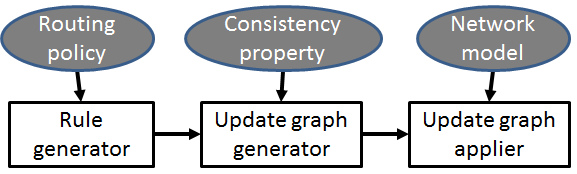
\includegraphics[width=\columnwidth]{figures/arch.png}\\
  \caption{Proposed architecture}\label{fig:arch}
\end{figure}


%In general, software defined networks should not be modeled by mere rules or rule changes, but rather by \emph{rule dependencies}. As we showed in this paper, rules changes often depend on each other, before a new rule can be used, one must make sure that other rules are already in place, or that other rules are being removed. These rule dependencies in general form a directed graph we call the dependency graph, as follows: The nodes of the dependency graph are rule changes, e.g. insert, remove, or change a rule at some node. These nodes are connected by directed edges that represent dependencies between rule changes. If a node does not have an edge pointing to it, the rule can be implemented immediately.

We propose an alternative architecture (Figure~\ref{fig:arch}) with three parts, one for each concern above: $i)$ the {\em rule generator} produces policy-compliant rules; $ii)$ the {\em update plan generator} produces a plan for applying those rules in a way that ensures consistency; and $iii)$  the {\em plan optimizer and executor} executes the plan efficiently.\footnote{In analogy to programs, compilers, and runtimes, the first part declaratively specifies the desired network state, the second produces instructions to safely update the network, and the third part executes the instructions efficiently, taking into account the properties of the underlying hardware.}

We represent the update plan using an {\em update DAG} (directed acyclic graph) in which nodes are updates (i.e., rule additions, deletions, or changes) and directed edges are dependencies between updates. Updates that do not have an inbound edge can be implemented immediately.

Using only updates as nodes does not capture all types of dependencies. Safe application of some updates requires time delays; e.g., in ~\cite{safeupdate}, rules with old version numbers can be removed only after time to drain in-transit packets has elapsed. Further, some updates may have dependencies such that they can be applied when any one of their parents have been applied; e.g., switch the rules of node $u$ in Figure \ref{fig:minimal} such that $u.old = w$ and $u.new = d$. Then, in order to prevent a loop, node $v$ must wait  for either $u$ \emph{or} $w$, not both.
%it does not need to wait for both, and we shouldn't make it wait for both when applying updates.

%
%Depending on the application, one may add several special nodes to increase the functionality of the dependency graph. A general problem are slow packets in transit. For instance, the packet coherence protocol by Reitblatt et al.~\cite{safeupdate} may remove old rules while packets using these rules are in still transit. Concretely, consider a packet $p$ in transit from $y$ to $x$ in the example of Figure \ref{fig:example}. If node $x$ already passed the last step of the consistency protocol~\cite{safeupdate} and removed the old rule when receiving packet $p$, node $x$ has not other option than dropping packet $p$ once it arrives. A simple technique to deal with packets in transit is adding reasonable timers before removing old rules, i.e. by adding a node in the dependency graph that demands to ``wait 10 seconds'' that points to the node that removes the old rule.

%Also, sometimes nodes that incorporate logical functions may be helpful. As an example, switch the rules of node $u$ in Figure \ref{fig:minimal}, such that $u.old = w$ and $u.new = d$. Then, in order to prevent a loop, node $v$ must wait, but node $v$ may wait for either node $u$ \emph{or} node $w$. In the dependency graph, one may now choose to include either the dependency between $u$ and $v$, or the dependency between $w$ and $v$. Even though both are correct, the dependency graph allows a better solution, as we can just include an ``or'' node, connecting the insertions of the new rules at $u$ and $w$ with the new rule at $v$, and then $v$ just needs to wait for the faster of $u$ and $w$.

To generally handle such dependencies, we introduce {\em combinator nodes} into the update DAG. Current combinators include delay and logical functions. A delay combinator is considered applied (i.e., its dependent updates can be now applied) after the specified time has elapsed since its parent updates were applied. A logical combinator is a logical function (e.g., AND or OR) over the binary state (applied or not) of its parents. It is considered applied when the function evaluates to true. These two combinators suffice to efficiently represent update plans for all procedures in Table~\ref{tbl:big}; future work may uncover the need for additional combinators.

\paragraphb{The update plan generator} proceeds in two steps. It first computes, using the old rules, new rules, and the desired consistency property, a {\em rule dependency graph} where nodes correspond to deletion of old rules or addition of new rules. It then converts this graph into an update DAG such that, starting from the old rules, applying the DAG leads to new rules.

This second step is straightforward if the graph is cycle-free; otherwise, we must break cycles. How this should be done depends on the consistency property, but a few general tools exist. One is using version numbers~\cite{safeupdate}, which help when a new rule must wait for an old rule to be removed. Introducing version numbers makes it clear which of the (otherwise) conflicting rules should be used. As an extension, if one is not willing to wait for a rule to be inserted, additional information (similar to source routing) may be embedded in the packet as to how it should be handled downstream  and the circular dependency vanishes.

Another tool for breaking cycles is using {\em helper updates}, which exist in neither the old or new rule sets but help with consistent updates. SWAN's staged partial moves~\cite{swan} can be expressed using helper updates that move subsets of flows to avoid overloading any link. Circularity due to prefix-based routing (\S\ref{sec:multidest}) can also be broken using helper updates. In Figure \ref{fig:multidest}, we can eliminate the cycle by breaking a single (default) rule into one for each of the two destinations covered by the default rule, introducing these rules during the update process and then removing them later.

%
%However, the main reason for dependency graphs is that they allow for a general understanding of the consistency of SDN updates. First, as our prefix routing example in Section \label{ref:multidest} showed, dependencies might have cycles, and a dependency graph is a perfect means to understand these cycles in a formal way. One might decide to eliminate these cycles by simply removing dependency edges, with the advantage to completely understand that exactly these removed consistency properties will be violated by doing so. But one can also handle cycles without violating consistency. In the example in Figure \ref{fig:multidest}, for instance, one can eliminate the cycle by breaking a single (default) rule into one for each of the two destinations covered by the default rule. TODO: describe details if needed?

%Another technique to eliminate cycles is to introduce version numbers. Version numbers in particular help if a rule needs to wait for another rule to be removed first. Just introduce a version number, and then it is clear which of the (otherwise) conflicting rules should be used. What if one is not willing to wait for a rule to be inserted? Just include the additional information in the packet, similarly to source routing, and the dependency is vanishes.

\paragraphb{The plan executor} applies the update DAG correctly and quickly. In deciding the order and timing of updates, it needs to factor in several concerns, including the delays from the controller to the switch, the mean and variance of the time a switch takes to apply an update, and limiting load on a switch. Further, in some cases, the update DAG may contain a long chain of dependencies. In the worst case, with $n$ nodes in the network, the chain can be $O(n)$ long (e.g., ensuring loop freedom for changing direction in a ring network.)
%and $O(n^2)$ single-hop messages will be needed because it can take $O(n)$ such messages for a switch and controller to communicate.
Long chains may be shortened, for instance, using version numbers.  Alternatively, we may also introduce a new primitive in switches by which a switch informs its dependents when it is safe to apply an update, which would enable updates to be done without $O(n)$ round trip exchanges with the controller. Developing efficient algorithms for applying update DAGs, while accounting for all these concerns, is a rich area for future work.

Sometimes, in the middle of forwarding state changes, we may need to change the network to yet another state (e.g., due to a failures). Such events are easier to handle in our architecture. The rule generator can compute the new state of the network, without worrying about the current, transient state. The plan executor knows the current state of the network, with some small uncertainty that corresponds to update messages that have been sent to the switches but have not been acknowledged. Using this state as the starting point, the plan generator can generate a new update DAG, which may cancel out updates in the old DAG. Then, the plan executor can start applying this new update DAG.


%The other main reason for dependency graphs is efficiency: Not only do they allow for a better understanding of minimal dependencies as shown in Section \ref{fig:minimal}. Also they provide a solid basis for optimizations. For instance, there are dependency graph that inevitably will contain a long chain of dependencies, and version numbers and other techniques help flattening such dependency graphs. For the sake of concreteness, consider a $n$-node network with a ring topology. In the old regime, all nodes point clockwise to destination $d$. In the new regime, all nodes point counter-clockwise to destination $d$. Let us call clockwise neighbor of $d$ node $u_1$, the clockwise neighbor of $u_i$ is node $u_{i+1}$. In other words, the counter-clockwise neighbor of $d$ is node $u_{n-1}$. In this example, the dependency graph for loop freedom is a linked list $u_1,u_2,\ldots,u_{n-1}$. If the dependency graph is synchronized with an SDN controller, no matter where in the ring network the SDN controller is located, $\Theta(n^2)$ messages are going to be transmitted before the network converged to the new solution. For loop freedom, this is the worst example, as the dependency graph for a single destination cannot be worse than a linked list. In such a case, it is possible to speed up conversion by using sequence numbers, or by having nodes informing neighbors directly, without going through the SDN controller. In both cases, the update can be performed using $O(n)$ messages only.

%So, the general procedure is as follows: First, the new rules are used to compute a dependency graph. This graph is then checked for cycles, which are eliminated using various techniques such as rule splitting or version numbers. Then the resulting cycle-free dependency graph (DAG) is fed into an optimizer, which speeds up conversion at the cost of introducing more memory, version numbers, direct update information between nodes, source routing, helper nodes, or other mechanisms. We end up with a flat dependency DAG, which can be directly implemented in the network.

%TODO: safeupdate is more parallel, however, using optimizations, dependencies do not have to be sequential, and can be optimized.

\section{Preliminary evaluation}
\label{sec:eval}

We have a preliminary implementation of the architecture above. Our focus thus far has been loop freedom and the update DAGs that emerge for it. In one experiment, we took Rocketfuel ISP topologies with intra-domain routing weights~\cite{rocketfuel-weights}. We considered link failures in these topologies, and our goal was loop free network updates from pre- to post-failure least-cost routing.

Figure~\ref{fig:as} plots the distribution of the length of dependency chains that emerge across ten trials, where a randomly selected link was failed in each, and update DAGs were computed using the procedure in \S\ref{sec:minimal}. We see that roughly half of the updates depend on 0 or 1 other switch, and 90\% of all rules are dependent on at most 3 other switches. In contrast, had we used Reitblatt's procedure~\cite{safeupdate}, which ensures the stronger property of packet coherence, rules would have had to wait for all other switches (well over a hundred in some cases), and a single slow switch can impede everyone.

We also see a small fraction of cases with chain lengths greater than 5. These are prime candidates for implementation through localized chain shortening optimizations by the plan executor.

% (and the plan generator can exclusively focus on maintaining loop freedom)


\begin{figure}[t!]
  \centering
  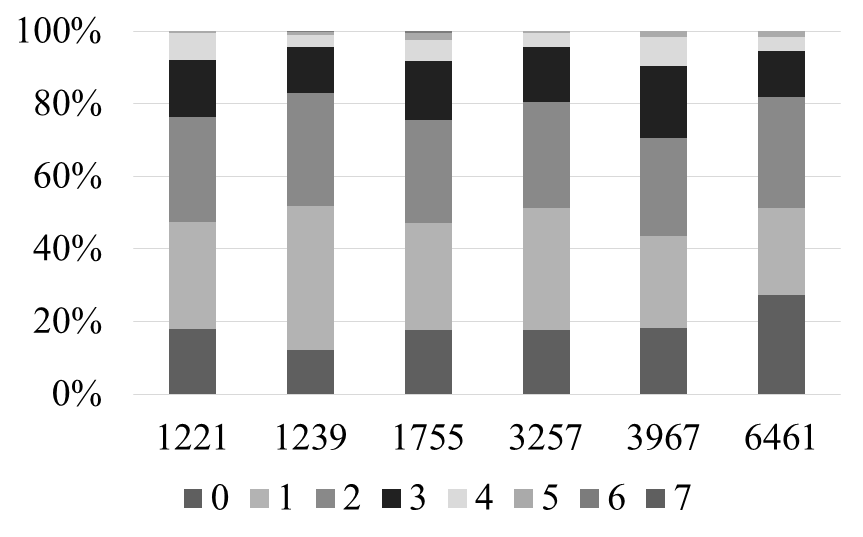
\includegraphics[width=2.5in]{figures/as.png}
  \vspace{-10pt}
  \caption{Chain lengths in update DAGs in six Rocketfuel topologies. The $x$-axis label denotes the ASN.}\label{fig:as}
\end{figure}

%Some additional snippets:
%
%The nodes in this graph are rules and they point to other rules that must be updated before them to guarantee loop freedom. While these graphs can be computed using an algorithm similar to the one above \ratul{true? need more details -- }, we cannot use the same update procedure that goes from roots to leafs. Instead, special care is needed for updating portions of the graph that form cycles.
%
%Nodes in a cycle can be updated in two ways. The first is using Reitblatt's procedure, which relies in version numbers for "atomically switching" a set of nodes. Another is to "break the cycles" by using helper rules that control subsets of the address space, thus removing the overlap. In the example above, \ratul{finish}.
%
%Which of the two methods is preferable depends on the context and other procedures may exist as well.
%
%Let's analyze it. There are only two reasons why we need network algorithms and protocols and the first place, first failures, second changes in either demand or infrastructure; if everything would be stable forever, there is no need to react (have protocols). In this work we essentially concentrate on the second (changes which can be planned). The first is also interesting, but mostly beyond the scope of this work. (This is where Ratul disagrees, and he is probably right.)
%
%Problem: Reaction time to failures and updates. A central controller is often slower than a distributed protocol, as it might be farther away, and the source of the problem/change is often close to those components that are most affected by a problem/change. Nevertheless, that’s again a failure problem. Is the only reason to use distributed protocols failure handling?
%
%(This is what this paper is about.) The answer is no. There is also synchronization. Even in the absence of failures, one cannot have nodes of a network migrate to a new version of operation at the very same instant. In theory, the last statement is trivial. In practice, clearly one tries to get as close as possible to optimal synchronization. Clearly, having an SDN helps a lot, as migration in heterogeneous networks is a whole different battle (this is another thing we discussed), as global updates of standard protocols show. However, even if the system is homogeneous, (time) synchronization is difficult [firing squad, or clock synchronization].
%
%Synchronization is an overloaded term, unfortunately. On the one hand we have something like (physical) clock synchronization, on the other hand we have (logical) synchronization. Perfect physical synchronization is impossible, so people often do logical synchronization. This is also what we do here or in SWAN.
%
%Or, to put it differently, as nodes cannot all migrate to the new version at exactly the same instance (and packets might be in transit still, and what not), we need a way to do a ``save transition'' from the old to the new state.
%


%First, what happens if the network is in the middle of a transition, and the SDN controller decides to update some rules (that might or might not have been rolled out already)? This can be integrated easily in the algorithm described above. In a nutshell, we just need to consider all rules that are possibly still existing in the network as old rules. As such, a node $u$ may have several old rules, pointing to different neighbors, plus one new rule. If some node $u$ was in limbo state before the new update was rolled out, it may have used either its old rule, or the intermediate rule (formerly known as new rule, now overwritten by the new rule). We know that mixing old and intermediate rules did not cause any loops, and as such we can treat both of them as old rules. If some rules have already been deleted, or have not been initiated, they can be ignored. Note that our algorithm also works in the presence of a whole set of old rules, and as such, it can automatically handle updates that interrupt transitions.

%A main cause for interrupting updates may be failures at nodes or edges. Essentially, failures may be handled in a standard way, by simply rolling out another batch of rules that will fix the failures. However, there is one exception, which we will first describe with an example: If some link $l$ is considered to be down, new rules will be introduced to route around this failed link $l$. An old rule on link $l$ might have a loop with some of the new rules, and as such the algorithm cannot push the new rules before the old rule is removed. Even worse, if the node $u$ holding the old rule is not accessible, the algorithm will not be able to push the fixing rules before node $u$ is reachable again. The SDN controller has a conflict of interest, it needs to quickly push a fix which must ignore (delete) the old rule, however, if unreachable node $u$ comes up again while doing so, the existing old rule will introduce a loop. (TODO: must be re-written, I just wanted to describe the problem.)


%Some additional snippets:
%
%Let’s analyze it. There are only two reasons why we need network algorithms and protocols and the first place, first failures, second changes in either demand or infrastructure; if everything would be stable forever, there is no need to react (have protocols). In this work we essentially concentrate on the second (changes which can be planned). The first is also interesting, but mostly beyond the scope of this work. (This is where Ratul disagrees, and he is probably right.)
%
%Problem: Reaction time to failures and updates. A central controller is often slower than a distributed protocol, as it might be farther away, and the source of the problem/change is often close to those components that are most affected by a problem/change. Nevertheless, that’s again a failure problem. Is the only reason to use distributed protocols failure handling?
%
%(This is what this paper is about.) The answer is no. There is also synchronization. Even in the absence of failures, one cannot have nodes of a network migrate to a new version of operation at the very same instant. In theory, the last statement is trivial. In practice, clearly one tries to get as close as possible to optimal synchronization. Clearly, having an SDN helps a lot, as migration in heterogeneous networks is a whole different battle (this is another thing we discussed), as global updates of standard protocols show. However, even if the system is homogeneous, (time) synchronization is difficult [firing squad, or clock synchronization].
%
%Synchronization is an overloaded term, unfortunately. On the one hand we have something like (physical) clock synchronization, on the other hand we have (logical) synchronization. Perfect physical synchronization is impossible, so people often do logical synchronization. This is also what we do here or in SWAN.
%
%Or, to put it differently, as nodes cannot all migrate to the new version at exactly the same instance (and packets might be in transit still, and what not), we need a way to do a ``save transition'' from the old to the new state.
%
%[Roger removed this missing snippet and used it in 4]
%
%Apart from time, there is also a space component, as we want to remove old rules as soon as possible (as soon as not used anymore).
%
%In this paper we discuss what the ``safe'' in safe transition is.
%
%We also discuss whether there is a tradeoff speed and safety.
%
%We exemplarily look into this tradeoff in one specific example (by looking at different ways to do such a transition).
%Some new ideas from discussions:
%
%What helper tools do you have? ``Just control network'' (including gateway routers, but not servers). If needed, one can add header, or mess with TTL. Also: Only talk to neighbors, or able to route messages?
%
%Other consistencies: FIFO, no drop, ``eventual'', suffix.
%
%Worst-case view: If there is a network/traffic pattern with a problem, then the consistency has a problem.
%
%You do not control old and new, so old=new is not a consistency criterion.
%
%
